\documentclass{TDP005mall}

\usepackage{enumitem}
\usepackage{graphicx}
\usepackage{float}


\newcommand{\version}{Version 1.1}
\author{Albin Dahlén, \url{albda746@student.liu.se}\\
  Filip Ingvarsson, \url{filin764@student.liu.se}}
\title{Kravspecifikation}
\date{2022-11-21}
\rhead{Albin Dahlén\\
Filip Ingvarsson}



\begin{document}
\projectpage
\section{Revisionshistorik}
\begin{table}[!h]
\begin{tabularx}{\linewidth}{|l|X|l|}
\hline
Ver. & Revisionsbeskrivning & Datum \\\hline
1.0 & Första utkast & 22-11-14 \\\hline
1.1 & Förändrat efter semenarie & 22-11-21 \\\hline
\end{tabularx}
\end{table}


\section{Spelidé}
Spelet kommer utspela sig i en 2D-värld med ett fågelperspektiv. En spelare ska styra en karaktär som attackeras av fiender.
Fienderna kommer försöka döda spelaren och spelaren i sin tur försvarar sig genom att döda fienderna. Karaktären styrs genom piltangenterna.
Spelaren kommer använda olika typer av vapen som kan bytas ut och eller uppgraderas under spelets gång. Fienderna kommer anfalla i olika 'vågor' som ökar i storlek och frekvens desto längre spelet har spelats.
Det finns olika typer av fienden där de olika typerna har olika hastighet,attackskada, liv och andra specialförmågor. Det finns även olika typer av banor där banans utseende kan försvåra eller förenkla spelet.

Spelet genererar även ett highscore beroende på hur väl man klarat spelet.


\section{Målgrupp}
Spelet riktar sig till personer som gillar shoot 'em spel och möjligheten att tävla med andra genom highscores.

\section{Spelupplevelse}
Spelet kommer vara utmanande och har stor återspelbarhet där man kan testa olika vapen och olika uppgraderingar.
Spelet kan även spelas om flera gånger för att försöka slå sitt eget eller sina vänners highscore.

\section{Spelmekanik}
Spelaren kommmer röra sig i spelet genom piltangenter, man kan byta dessa knappar i menyn.
\begin{table}[H]
  \begin{center}
  \begin{tabular}{ |c|c| } 
    \hline
    \textbf{Tangentknapp} & \textbf{Åtgärd} \\
    \hline
    → & Flytta spelaren åt höger \\
    \hline
    ↓ & Flytta spelaren neråt \\
    \hline
    ← & Flytta spelaren åt vänster \\
    \hline
    ↑ & Flytta spelaren uppåt \\
    \hline
    Mouse button 1 & Använd vapen \\
    \hline
  \end{tabular}
  \end{center}
  \caption{Keybindings}
  \label{tab:movement}
\end{table}

\section{Regler}
\subsection{Spelplan}
\begin{itemize}
\item Hinder på spelplanen slumpas fram.
\item Spelplanen har en fixerad storlek.
\end{itemize}

\subsection{Spelare}
\begin{itemize}
\item Spelaren är den figur som användaren styr.
\item Spelaren kan använda sitt vapen för att skada fiendeobjekt.
\item Spelaren kan röra sig uppåt, neråt, höger och vänster.
\item Spelaren startar i mitten av spelplanen när spelet startar.
\item Spelaren börjar med 100 i hälsa.
\item Spelaren kan kollidera med fiender.
\item Spelaren kan kollidera med hinder på spelplanen.
\item Spelaren förlorar hälsa vid kollision med en fiende.
\item Spelaren kan inte röra sig utanför spelplanen.
\item När spelaren har 0 eller minder i hälsa avslutas spelet.
\end{itemize}


\subsection{Fiendetyper}

\subsubsection{Fiende typ 1}
\begin{itemize}
\item Rör sig alltid mot spelaren.
\item Har 100 i hälsa.
\item Skadar spelaren med 10 enheter.
\item Rörelsehastighet: mellan.
\end{itemize}

\subsubsection{Fiende typ 2}
\begin{itemize}
\item Rör sig alltid mot spelaren.
\item Har 50 i hälsa.
\item Skadar spelaren med 10 enheter.
\item Rörelsehastighet: snabb.
\end{itemize}

\subsection{Poäng}
Poäng erhålles vid dödandet av fiender och antal avklarade vågor.

\subsection{Projektilregler}
Projektiler färdas i den riktning som muspekaren är i jämfört med spelaren.
Projektilen ska kunna kollidera med fiender.
När projektilen kolliderar med en fiende eller når slutet av spelplanen ska projektilen försvinna.
Om projektilen kolliderar med en fiende ska fienden ta skada.

\section{Visualisering}

\begin{figure}[H]
  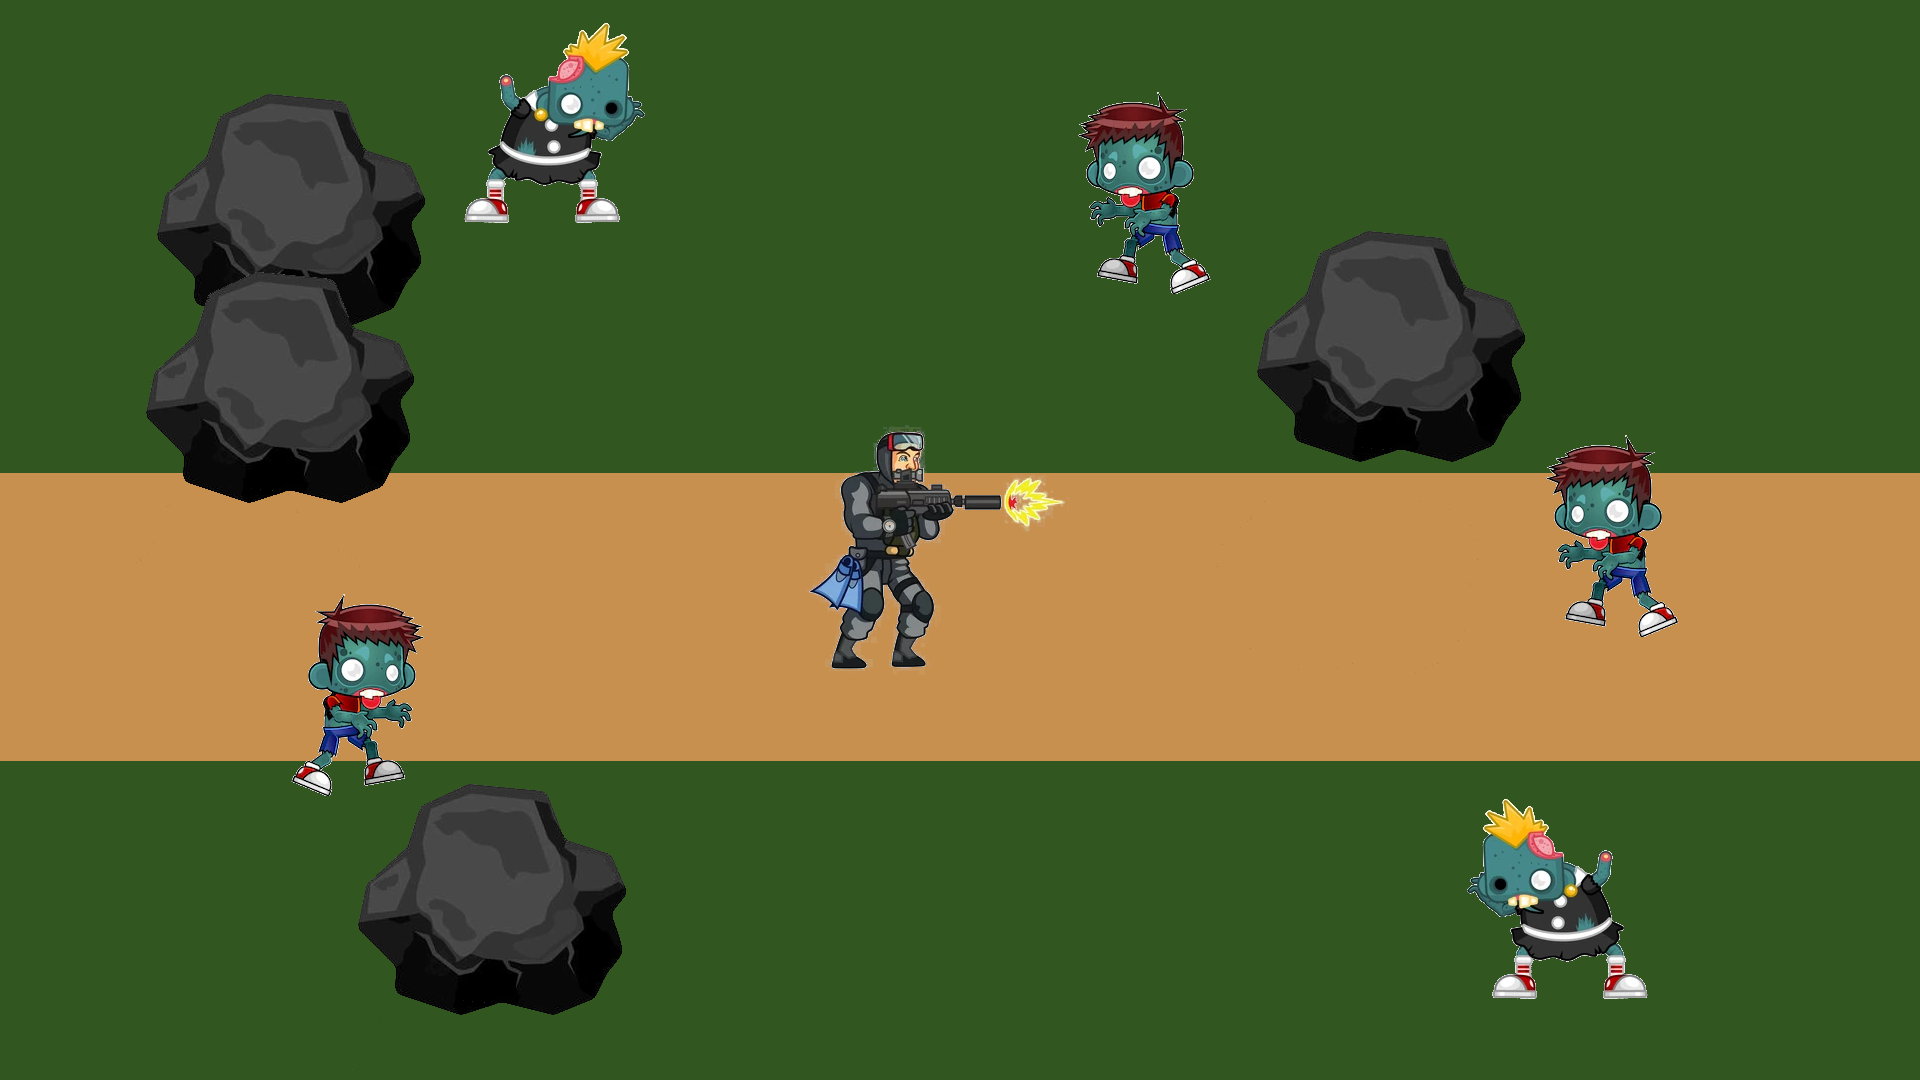
\includegraphics[width=\linewidth]{test.png}
  \caption {En prototypbild av spelet}
  \label {fig:picture}
\end {figure}

\section{Kravformulering}
\subsection{Ska-krav}
\begin{enumerate}[label=S\arabic*]
\item Det skall finnas en startmeny där spelaren kan välja att spela eller avsluta spelet.
\item Spelaren ska med hjälp av piltangenterna kunna förflytta spelarobjektet enligt tabell \ref{tab:movement}.
\item Det ska finnas 2 olika typer av fiendeobjekt.
\item Fiendeobjekten ska förflytta sig mot spelaren.
\item Om fiendeobjektet kolliderar med spelaren ska spelarens hälsa minska med x enheter beroende på vilken fiende typ det var.
\item Spelaren ska ha ett projektilvapen.
\item Om spelaren träffar fienden med en projektill ska fienden ta skada.
\item När ett fiendeobjekt når 0 eller mindre i hälsa ska objektet dö.
\item Om spelarens hälsa når 0 eller mindre ska spelet avslutas och game over visas.
\item En tvådimensionell spelplan ska ritas ut på skärmen och ska täcka hela spelfönstret.
\item Spelplanens uteseende slumpas fram.
\item Det ska finnas flera instanser av varje fiendeobjekt.
\item När spelaren dödar en fiende ska poäng erhållas.
\end{enumerate}

\subsection{Bör-krav}
\begin{enumerate}[label=B\arabic*]
\item Startmenyn ska ha ett alternativ för att ändra keybindings.
\item Vapen ska kunna uppgraderas.
\item När spelaren dödar en fiende ska experince points erhållas.
\item Fiendeobjekten ska ha olika förflyttningsmönster.
\item Det ska finnas olika typer av attacker för fiendeobjekten.
\item Det finns hinder som spelar- och fiendeobjekten kan kollidera med.
\end{enumerate}

\section{Kravuppfyllelse}

\subsection{Spelet ska simulera en värld som innehåller olika typer av objekt. Objekten ska ha olika beteenden och röra sig i världen och agera på olika sätt när de möter andra objekt.}
Uppfylles av krav S2, S3, S4, S5, S7, S8, S9.
\subsection{Det måste finnas minst tre olika typer av objekt och det ska finnas flera instanser av minst två av dessa. T.ex ett spelarobjekt och många instanser av två olika slags fiendeobjekt.}
Uppfylles av krav S2, S3, S4, S12.
\subsection{Ett beteende som måste finnas med är att figurerna ska röra sig över skärmen. Rörelsen kan följa ett mönster och/eller vara slumpmässig. Minst ett objekt, utöver spelaren ska ha någon typ av rörelse.}
Uppfylles av krav S2, S4. 
\subsection{En figur ska styras av spelaren, antingen med tangentbordet eller med musen. Du kan även göra ett spel där man spelar två stycken genom att dela på tangentbordet (varje spelare använder olika tangenter). Då styr man var sin figur.}
Uppfylles av krav S2.
\subsection{Grafiken ska vara tvådimensionell.}
Uppfylles av krav S10.
\subsection{Världen (spelplanen) kan antas vara lika stor som fönstret (du kan göra en större spelplan med scrollning, men det blir lite krångligare).}
Uppfylles av krav S10.
\subsection{Det ska finnas kollisionshantering, det vill säga, det ska hända olika saker när objekten möter varandra, de ska påverka varandra på något sätt. T.ex kan ett av objekten tas bort, eller så kan objekten förvandlas på något sätt, eller så kan ett nytt objekt skapas. (Ett exempel på att skapa/ta bort objekt är när man i Space Invaders trycker på skjuta-knappen, t.ex en musknapp, då avfyras ett laserskott och skottet blir då en ny figur som skapas och placeras i världen, på en position vid laserkanonens mynning. Skottet rör sig framåt (uppåt) och om det träffar ett fiendeskepp tas både skottet och skeppet bort, om skottet kommer utanför spelplanen, dvs det missar, tas det endast bort.)}
Uppfylles av krav S5, S7.
\subsection{Det ska vara enkelt att lägga till eller ändra banor i spelet. Detta kan exempelvis lösas genom att läsa in banor från en fil (lite som i Sokoban-labben i TDP002), eller genom att ha funktioner i programkoden som bygger upp en datastruktur som definierar en bana.}
Uppfylles av krav S11.
\subsection{Spelet måste upplevas som ett sammanhängande spel som går att spela!}
Uppfylles av alla krav.


\end{document}
